\section{Forward problem}


 An electrode position
consists of a letter and a number. What is the meaning of the letter? Do you see a
pattern in the evenness or oddness of the numbers? Mention this in your report

\begin{figure}[!htbp]
\centering
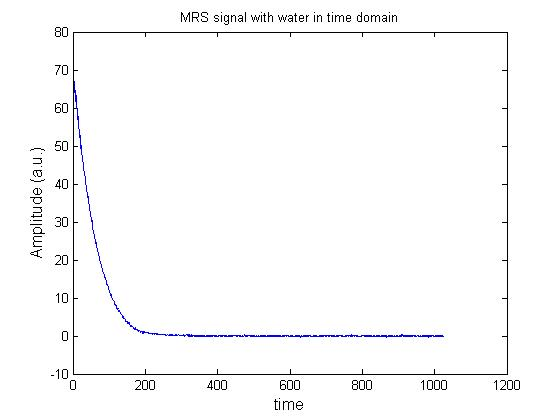
\includegraphics[width=.5\textwidth]{1.jpg}
\caption{Electrode placement in the head}
\end{figure}

Hereby the electrode placement in the brain is indicated. There is an arbitrary placement of the electrodes symmetric to the Cz electrode right in the middle of the head. The meaning of the letters is that 

Letters indicate that the frontal, lateral lone and prefrontal lobe, back lobe. Meaning that the signal letters have to be put very accurately in order to address the signals consistently to the lobes. In addition to being symmetric to the main electrode at the crown the electrodes even numbers are at left and right hand side and odd numbers upwards and downwards.

\begin{figure}[!htbp]
\minipage{.5\textwidth}%
\centering
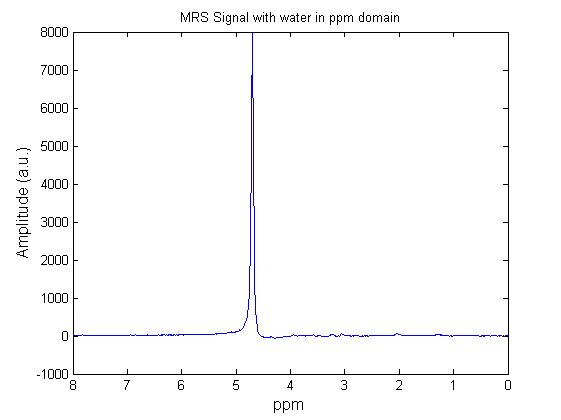
\includegraphics[width=1\textwidth]{2.jpg}
\subcaption{}
\endminipage\hfill
\minipage{.5\textwidth}%
\centering

\includegraphics[width=1\textwidth]{3.jpg}
\subcaption{}
\endminipage\hfill
\caption{Dipole placed between the center of the head and the righ ear}
\end{figure}
This is done with the command showdipole([x y z dx dy dz],hm) where x is the x coordinate starting from 0 up to 0.1.
For our requirements this coordinate in particular has to be 0.05 in order to put the dipole between the center and the right ear.
showdipole([.05 0 0 0 0 1],hm)

Forther more a dipole is placed at the center of the head as in figure \ref{a1} and the outcome voltage from this dipole is plotted in the map figure at \ref{a2}

\begin{figure}[!htbp]
\minipage{.5\textwidth}%
\centering
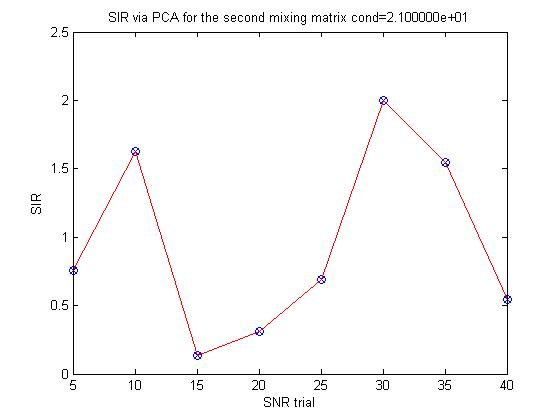
\includegraphics[width=1\textwidth]{4.jpg}
\subcaption{Voltage distribution along the electrodes}\label{a2}
\endminipage\hfill
\minipage{.5\textwidth}%
\centering
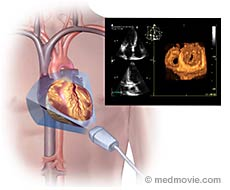
\includegraphics[width=1\textwidth]{5.jpg}
\subcaption{Dipole placed at the center}\label{a1}
\endminipage\hfill
\caption{Voltage distribution created from the central dipole}
\end{figure}


\begin{figure}[!htbp]
\minipage{.33\textwidth}%
\centering
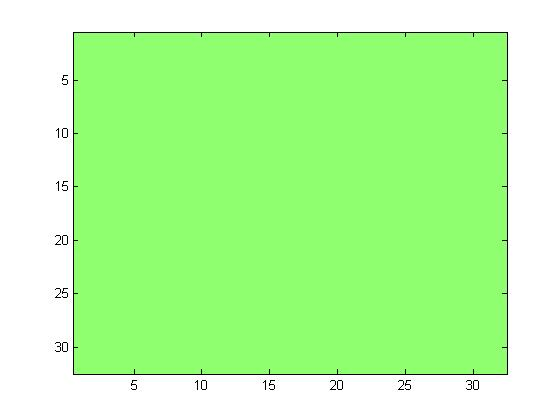
\includegraphics[width=1\textwidth]{6.jpg}
\subcaption{Lead field matrix along the x axis which is exactly as the the real voltage distribution of the main dipole}
\endminipage\hfill
\minipage{.33\textwidth}%
\centering
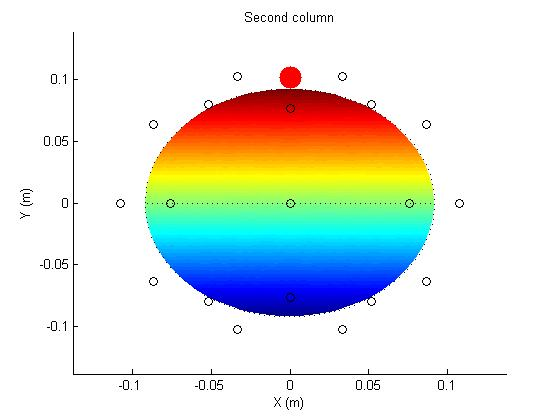
\includegraphics[width=1\textwidth]{7.jpg}
\subcaption{Lead filed matrix plot for the middle column along the y axis}
\endminipage\hfill
\minipage{.33\textwidth}%
\centering
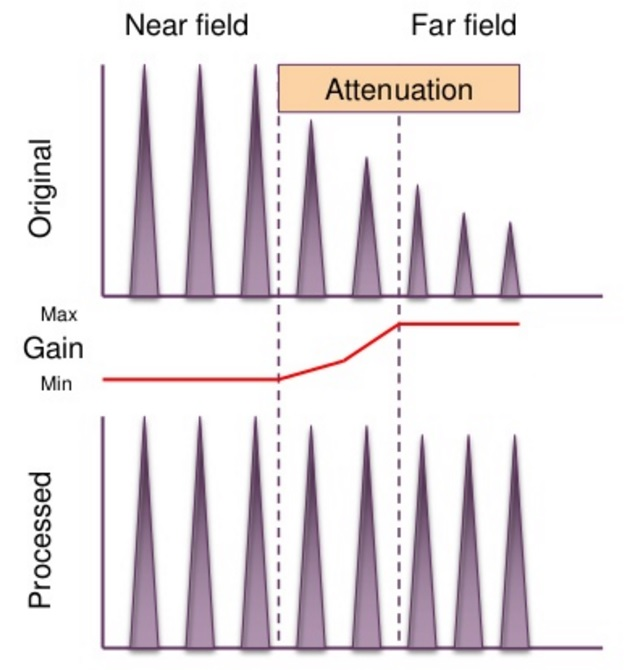
\includegraphics[width=1\textwidth]{8.jpg}
\subcaption{Lead filed matrix plot for the middle column along the y axis}
\endminipage\hfill
\caption{Lead field matrix plots respectively to the columns}
\end{figure}

Using the linearly of the Maxwell equation means that the pressure field total produced via two independent dipole will result in the sum of their receptive dipoles.In our case with two dipoles, one along the x axis and the other one along z axis. The result resulting voltage will have the maximum somewhere in skew between these two direction in other wards at the vectorial sum of this dipoles. 

\begin{figure}[!htbp]
\minipage{.5\textwidth}%
\centering
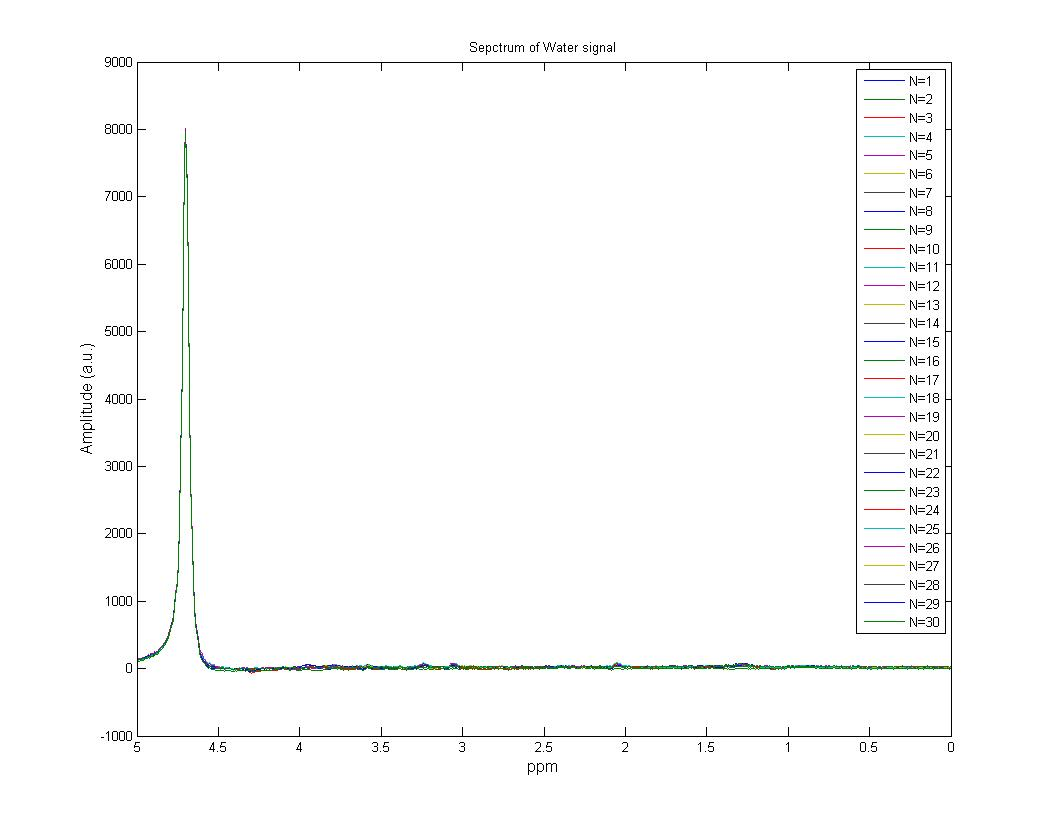
\includegraphics[width=1\textwidth]{9.jpg}
\subcaption{}
\endminipage\hfill
\minipage{.5\textwidth}%
\centering
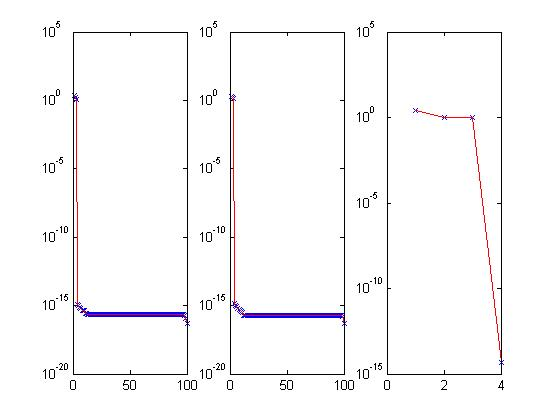
\includegraphics[width=1\textwidth]{10.jpg}
\subcaption{}
\endminipage\hfill
\caption{The voltage from both dipoles at the center where the first one directed along x the other one is oriented along z axis}
\end{figure}


\begin{figure}[!htbp]
\minipage{.5\textwidth}%
\centering
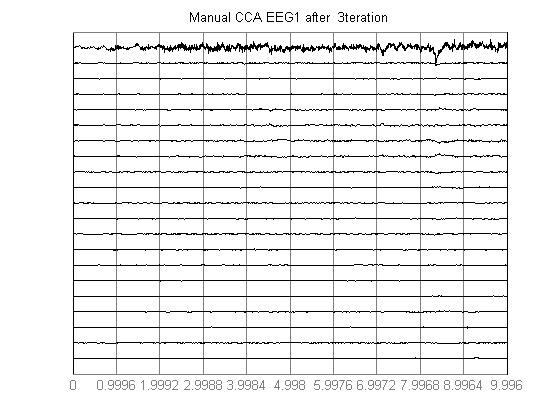
\includegraphics[width=1\textwidth]{11.jpg}
\subcaption{EEG simulated from the dipole placed at an arbitrary place in the brain rotating along xy plane }
\endminipage\hfill
\minipage{.5\textwidth}%
\centering
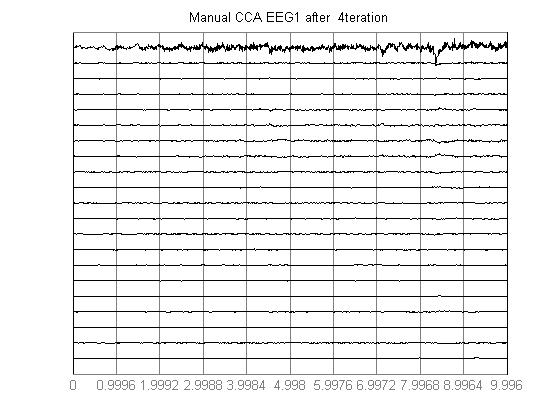
\includegraphics[width=1\textwidth]{12.jpg}
\subcaption{Dipole location and orientation in the brain}
\endminipage\hfill
\caption{EEG signal simulated via the rotating dipole int he xy plane}
\end{figure}

